% Conceptual framework diagram — original, drawn from this project's own
% architecture. Structurally inspired by JUNE-style layered ABM overview
% figures (a generative core with a visually separated analysis layer),
% but not copied from JUNE's text, box content, or visual design.
\documentclass[border=6pt]{standalone}
\usepackage{tikz}
\usetikzlibrary{arrows.meta, positioning, fit, backgrounds, shadows}

\begin{document}
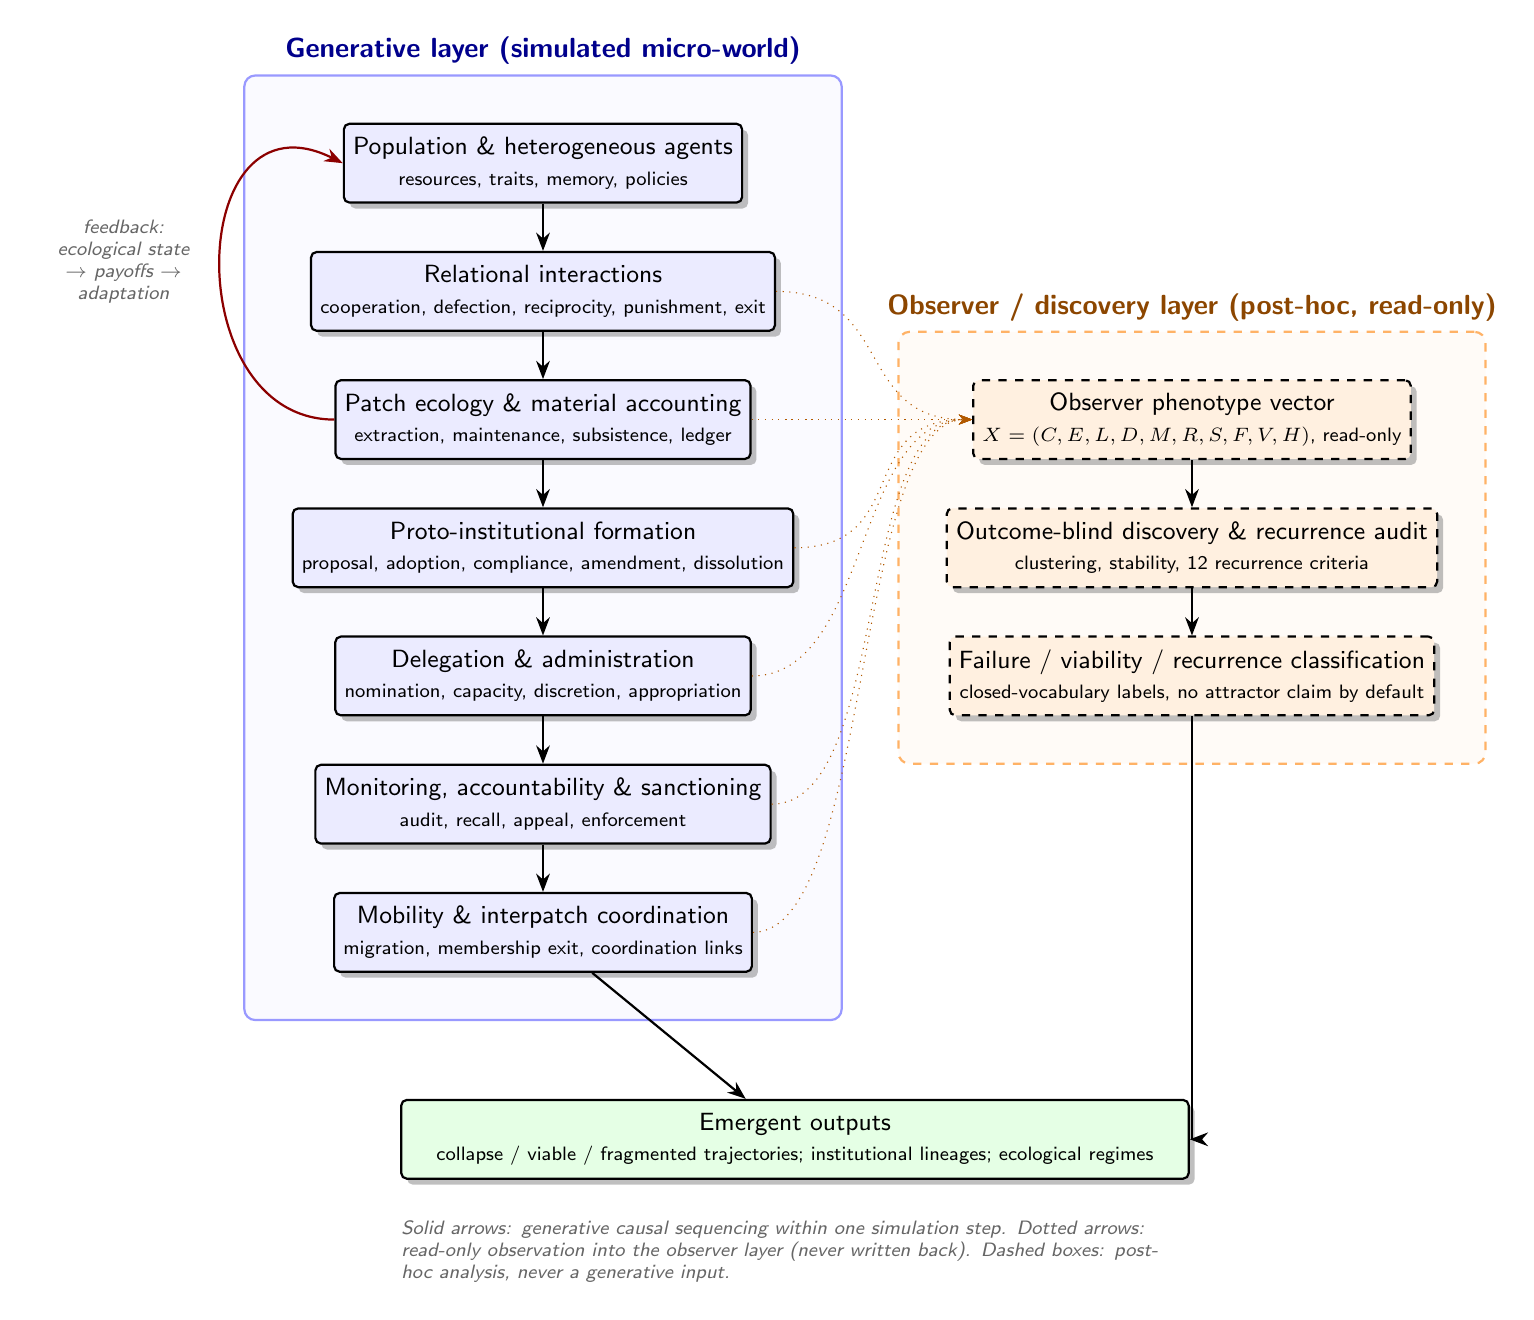
\begin{tikzpicture}[
    font=\sffamily\small,
    >=Stealth,
    node distance=6mm and 10mm,
    genbox/.style={draw, rounded corners=2pt, fill=blue!8, align=center,
        minimum width=48mm, minimum height=10mm, thick, drop shadow},
    obsbox/.style={draw, rounded corners=2pt, fill=orange!12, align=center,
        minimum width=48mm, minimum height=10mm, thick, dashed, drop shadow},
    outbox/.style={draw, rounded corners=2pt, fill=green!10, align=center,
        minimum width=100mm, minimum height=10mm, thick, drop shadow},
    lbl/.style={font=\sffamily\scriptsize\itshape, text=black!60},
]

% --- Generative layer stack ---
\node[genbox] (pop) {Population \& heterogeneous agents\\ \scriptsize resources, traits, memory, policies};
\node[genbox, below=of pop] (rel) {Relational interactions\\ \scriptsize cooperation, defection, reciprocity, punishment, exit};
\node[genbox, below=of rel] (eco) {Patch ecology \& material accounting\\ \scriptsize extraction, maintenance, subsistence, ledger};
\node[genbox, below=of eco] (inst) {Proto-institutional formation\\ \scriptsize proposal, adoption, compliance, amendment, dissolution};
\node[genbox, below=of inst] (del) {Delegation \& administration\\ \scriptsize nomination, capacity, discretion, appropriation};
\node[genbox, below=of del] (acc) {Monitoring, accountability \& sanctioning\\ \scriptsize audit, recall, appeal, enforcement};
\node[genbox, below=of acc] (mob) {Mobility \& interpatch coordination\\ \scriptsize migration, membership exit, coordination links};

% Generative-layer frame
\begin{scope}[on background layer]
\node[draw=blue!40, thick, rounded corners=4pt, fill=blue!2,
      fit=(pop)(rel)(eco)(inst)(del)(acc)(mob), inner sep=6mm,
      label={[font=\sffamily\bfseries, text=blue!55!black]above:Generative layer (simulated micro-world)}] (genframe) {};
\end{scope}

% --- Forward arrows down the stack ---
\draw[->, thick] (pop) -- (rel);
\draw[->, thick] (rel) -- (eco);
\draw[->, thick] (eco) -- (inst);
\draw[->, thick] (inst) -- (del);
\draw[->, thick] (del) -- (acc);
\draw[->, thick] (acc) -- (mob);

% --- Observer / discovery layer, visually separated to the right ---
\node[obsbox, right=28mm of eco] (phen) {Observer phenotype vector\\ \scriptsize $X=(C,E,L,D,M,R,S,F,V,H)$, read-only};
\node[obsbox, below=of phen] (disc) {Outcome-blind discovery \& recurrence audit\\ \scriptsize clustering, stability, 12 recurrence criteria};
\node[obsbox, below=of disc] (class) {Failure / viability / recurrence classification\\ \scriptsize closed-vocabulary labels, no attractor claim by default};

\begin{scope}[on background layer]
\node[draw=orange!60, thick, dashed, rounded corners=4pt, fill=orange!3,
      fit=(phen)(disc)(class), inner sep=6mm,
      label={[font=\sffamily\bfseries, text=orange!55!black]above:Observer / discovery layer (post-hoc, read-only)}] (obsframe) {};
\end{scope}

\draw[->, thick] (phen) -- (disc);
\draw[->, thick] (disc) -- (class);

% Read-only taps from generative state into the observer layer (never the reverse)
\foreach \g in {rel, eco, inst, del, acc, mob} {
  \draw[->, thin, orange!70!black, dotted] (\g.east) .. controls +(15mm,0) and +(-15mm,0) .. (phen.west);
}

% --- Emergent outputs, below both stacks, fed only from the generative layer ---
\node[outbox, below=16mm of mob, xshift=32mm] (out) {Emergent outputs\\ \scriptsize collapse / viable / fragmented trajectories; institutional lineages; ecological regimes};
\draw[->, thick] (mob) -- (out);
\draw[->, thick] (class) |- (out);

% --- Feedback path: ecological state shapes subsequent agent behaviour ---
\draw[->, thick, red!55!black] (eco.west) .. controls +(-20mm,0) and +(-20mm,10mm) .. (pop.west)
    node[midway, left, lbl, text width=22mm, align=center] {feedback:\\ ecological state $\rightarrow$ payoffs $\rightarrow$ adaptation};

% --- Legend note ---
\node[lbl, below=4mm of out, text width=100mm, align=left] {Solid arrows: generative causal sequencing within one simulation step. Dotted arrows: read-only observation into the observer layer (never written back). Dashed boxes: post-hoc analysis, never a generative input.};

\end{tikzpicture}
\end{document}
